\chapter*{Dodatak: Prikaz aktivnosti grupe}
		\addcontentsline{toc}{chapter}{Dodatak: Prikaz aktivnosti grupe}
		
		\section*{Dnevnik sastajanja}
		
		\begin{packed_enum}
			\item  sastanak
			
			\item[] \begin{packed_item}
				\item Datum: 13. listopada 2021.
				\item Prisustvovali: B.Kazazić, M.Erlić, B.Pavlović, A.Pašalić, L.Raspudić, P.Sušac, V.Žunar
				\item Teme sastanka:
				\begin{packed_item}
					\item 1. sastanak s asistentom i demonstratorom
					\item raščišćavanje nejasnoća
				\end{packed_item}
			\end{packed_item}
			
			\item  sastanak
			\item[] \begin{packed_item}
				\item Datum: 14. listopada 2021.
				\item Prisustvovali: B.Kazazić, M.Erlić, B.Pavlović, A.Pašalić, L.Raspudić, V.Žunar
				\item Teme sastanka:
				\begin{packed_item}
					\item ažuriranje LaTeX dokumentacije
					\item dodjela zadataka članovima tima
					\item platforme za komunikaciju
				\end{packed_item}
			\end{packed_item}
			
			\item  sastanak
			\item[] \begin{packed_item}
				\item Datum: 18. listopada 2021.
				\item Prisustvovali: B.Kazazić, M.Erlić, B.Pavlović, L.Raspudić, P.Sušac, V.Žunar
				\item Teme sastanka:
				\begin{packed_item}
					\item raspodjela zadataka
				\end{packed_item}
			\end{packed_item}
			
			\item  sastanak
			\item[] \begin{packed_item}
				\item Datum: 22. listopada 2021.
				\item Prisustvovali: B.Kazazić, M.Erlić, B.Pavlović, A.Pašalić, P.Sušac, V.Žunar
				\item Teme sastanka:
				\begin{packed_item}
					\item dodjela zadataka članovima tima
				\end{packed_item}
			\end{packed_item}
			%
			
		\end{packed_enum}
		
		\eject
		\section*{Tablica aktivnosti}
		
			\textbf{\textit{Kontinuirano osvježavanje}}\\
			
			 \textit{Napomena: Doprinose u aktivnostima treba navesti u satima po članovima grupe po aktivnosti.}
					
						
			
			\begin{longtabu} to \textwidth {|X[7, l]|X[1, c]|X[1, c]|X[1, c]|X[1, c]|X[1, c]|X[1, c]|X[1, c]|}
								
				\cline{2-8} \multicolumn{1}{c|}{\textbf{}} &     \multicolumn{1}{c|}{\rotatebox{90}{\textbf{Bernard Kazazić}}} & \multicolumn{1}{c|}{\rotatebox{90}{\textbf{Ante Pašalić}}} &	\multicolumn{1}{c|}{\rotatebox{90}{\textbf{Barbara Pavlović }}} &
				\multicolumn{1}{c|}{\rotatebox{90}{\textbf{Luka Raspudić }}} &	\multicolumn{1}{c|}{\rotatebox{90}{\textbf{Marijan Erlić}}} &
				\multicolumn{1}{c|}{\rotatebox{90}{\textbf{Petar Sušac }}} &	\multicolumn{1}{c|}{\rotatebox{90}{\textbf{Veronika Žunar }}} \\ \hline 
				\endfirsthead
				
			
				\cline{2-8} \multicolumn{1}{c|}{\textbf{}} &     \multicolumn{1}{c|}{\rotatebox{90}{\textbf{Bernard Kazazić}}} & \multicolumn{1}{c|}{\rotatebox{90}{\textbf{Ante Pašalić}}} &	\multicolumn{1}{c|}{\rotatebox{90}{\textbf{Barbara Pavlović }}} &
				\multicolumn{1}{c|}{\rotatebox{90}{\textbf{Luka Raspudić }}} &	\multicolumn{1}{c|}{\rotatebox{90}{\textbf{Marijan Erlić}}} &
				\multicolumn{1}{c|}{\rotatebox{90}{\textbf{Petar Sušac }}} &	\multicolumn{1}{c|}{\rotatebox{90}{\textbf{Veronika Žunar }}} \\ \hline 
				\endhead
				
				
				\endfoot
							
				 
				\endlastfoot
				
				Upravljanje projektom 		& 1600 &  &  &  &  &  &   \\ \hline
				Opis projektnog zadatka 	& &  & 100 & 100 &  & 60 & 100 \\ \hline
				
				Funkcionalni zahtjevi       &  & 30 &  &  &  & 45 &  \\ \hline
				Opis pojedinih obrazaca 	&  &  &  &  & 90 &  &  \\ \hline
				Dijagram obrazaca 			&  &  &  &  &  &  &  \\ \hline
				Sekvencijski dijagrami 		&  &  &  &  &  &  &  \\ \hline
				Opis ostalih zahtjeva 		&  &  &  &  & 60 &  &  \\ \hline

				Arhitektura i dizajn sustava	 &  &  &  &  &  &  &  \\ \hline
				Baza podataka				&  &  &  &  &  &  &   \\ \hline
				Dijagram razreda 			&  &  &  &  &  &  &   \\ \hline
				Dijagram stanja				&  &  &  &  &  &  &  \\ \hline
				Dijagram aktivnosti 		&  &  &  &  &  &  &  \\ \hline
				Dijagram komponenti			&  &  &  &  &  &  &  \\ \hline
				Korištene tehnologije i alati 		&  &  &  &  &  &  &  \\ \hline
				Ispitivanje programskog rješenja 	&  &  &  &  &  &  &  \\ \hline
				Dijagram razmještaja			&  &  &  &  &  &  &  \\ \hline
				Upute za puštanje u pogon 		&  &  &  &  &  &  &  \\ \hline 
				Dnevnik sastajanja 			&  &  &  &  & 120 &  &  \\ \hline
				Zaključak i budući rad 		&  &  &  &  &  &  &  \\  \hline
				Popis literature 			&  &  &  &  &  &  &  \\  \hline
				Izrada korisničkog sučelja			&  &  &  &  &  &  &  \\  \hline
				Izrada \textit{backend} aplikacije 			&  &  &  &  &  &  &  \\  \hline
				Postavljanje aplikacije na Heroku 	&  &  &  &  &  &  &  \\ \hline
				Pisanje LaTeX dokumentacije			&  &  &  &  &  &  &  \\  \hline
				
				
			\end{longtabu}
					
					
		\eject
		\section*{Dijagrami pregleda promjena}
		
% 		\textbf{\textit{dio 2. revizije}}\\
		
% 		\textit{Prenijeti dijagram pregleda promjena nad datotekama projekta. Potrebno je na kraju projekta generirane grafove s gitlaba prenijeti u ovo poglavlje dokumentacije. Dijagrami za vlastiti projekt se mogu preuzeti s gitlab.com stranice, u izborniku Repository, pritiskom na stavku Contributors.}
		
		\begin{figure}[H]
					\centering
					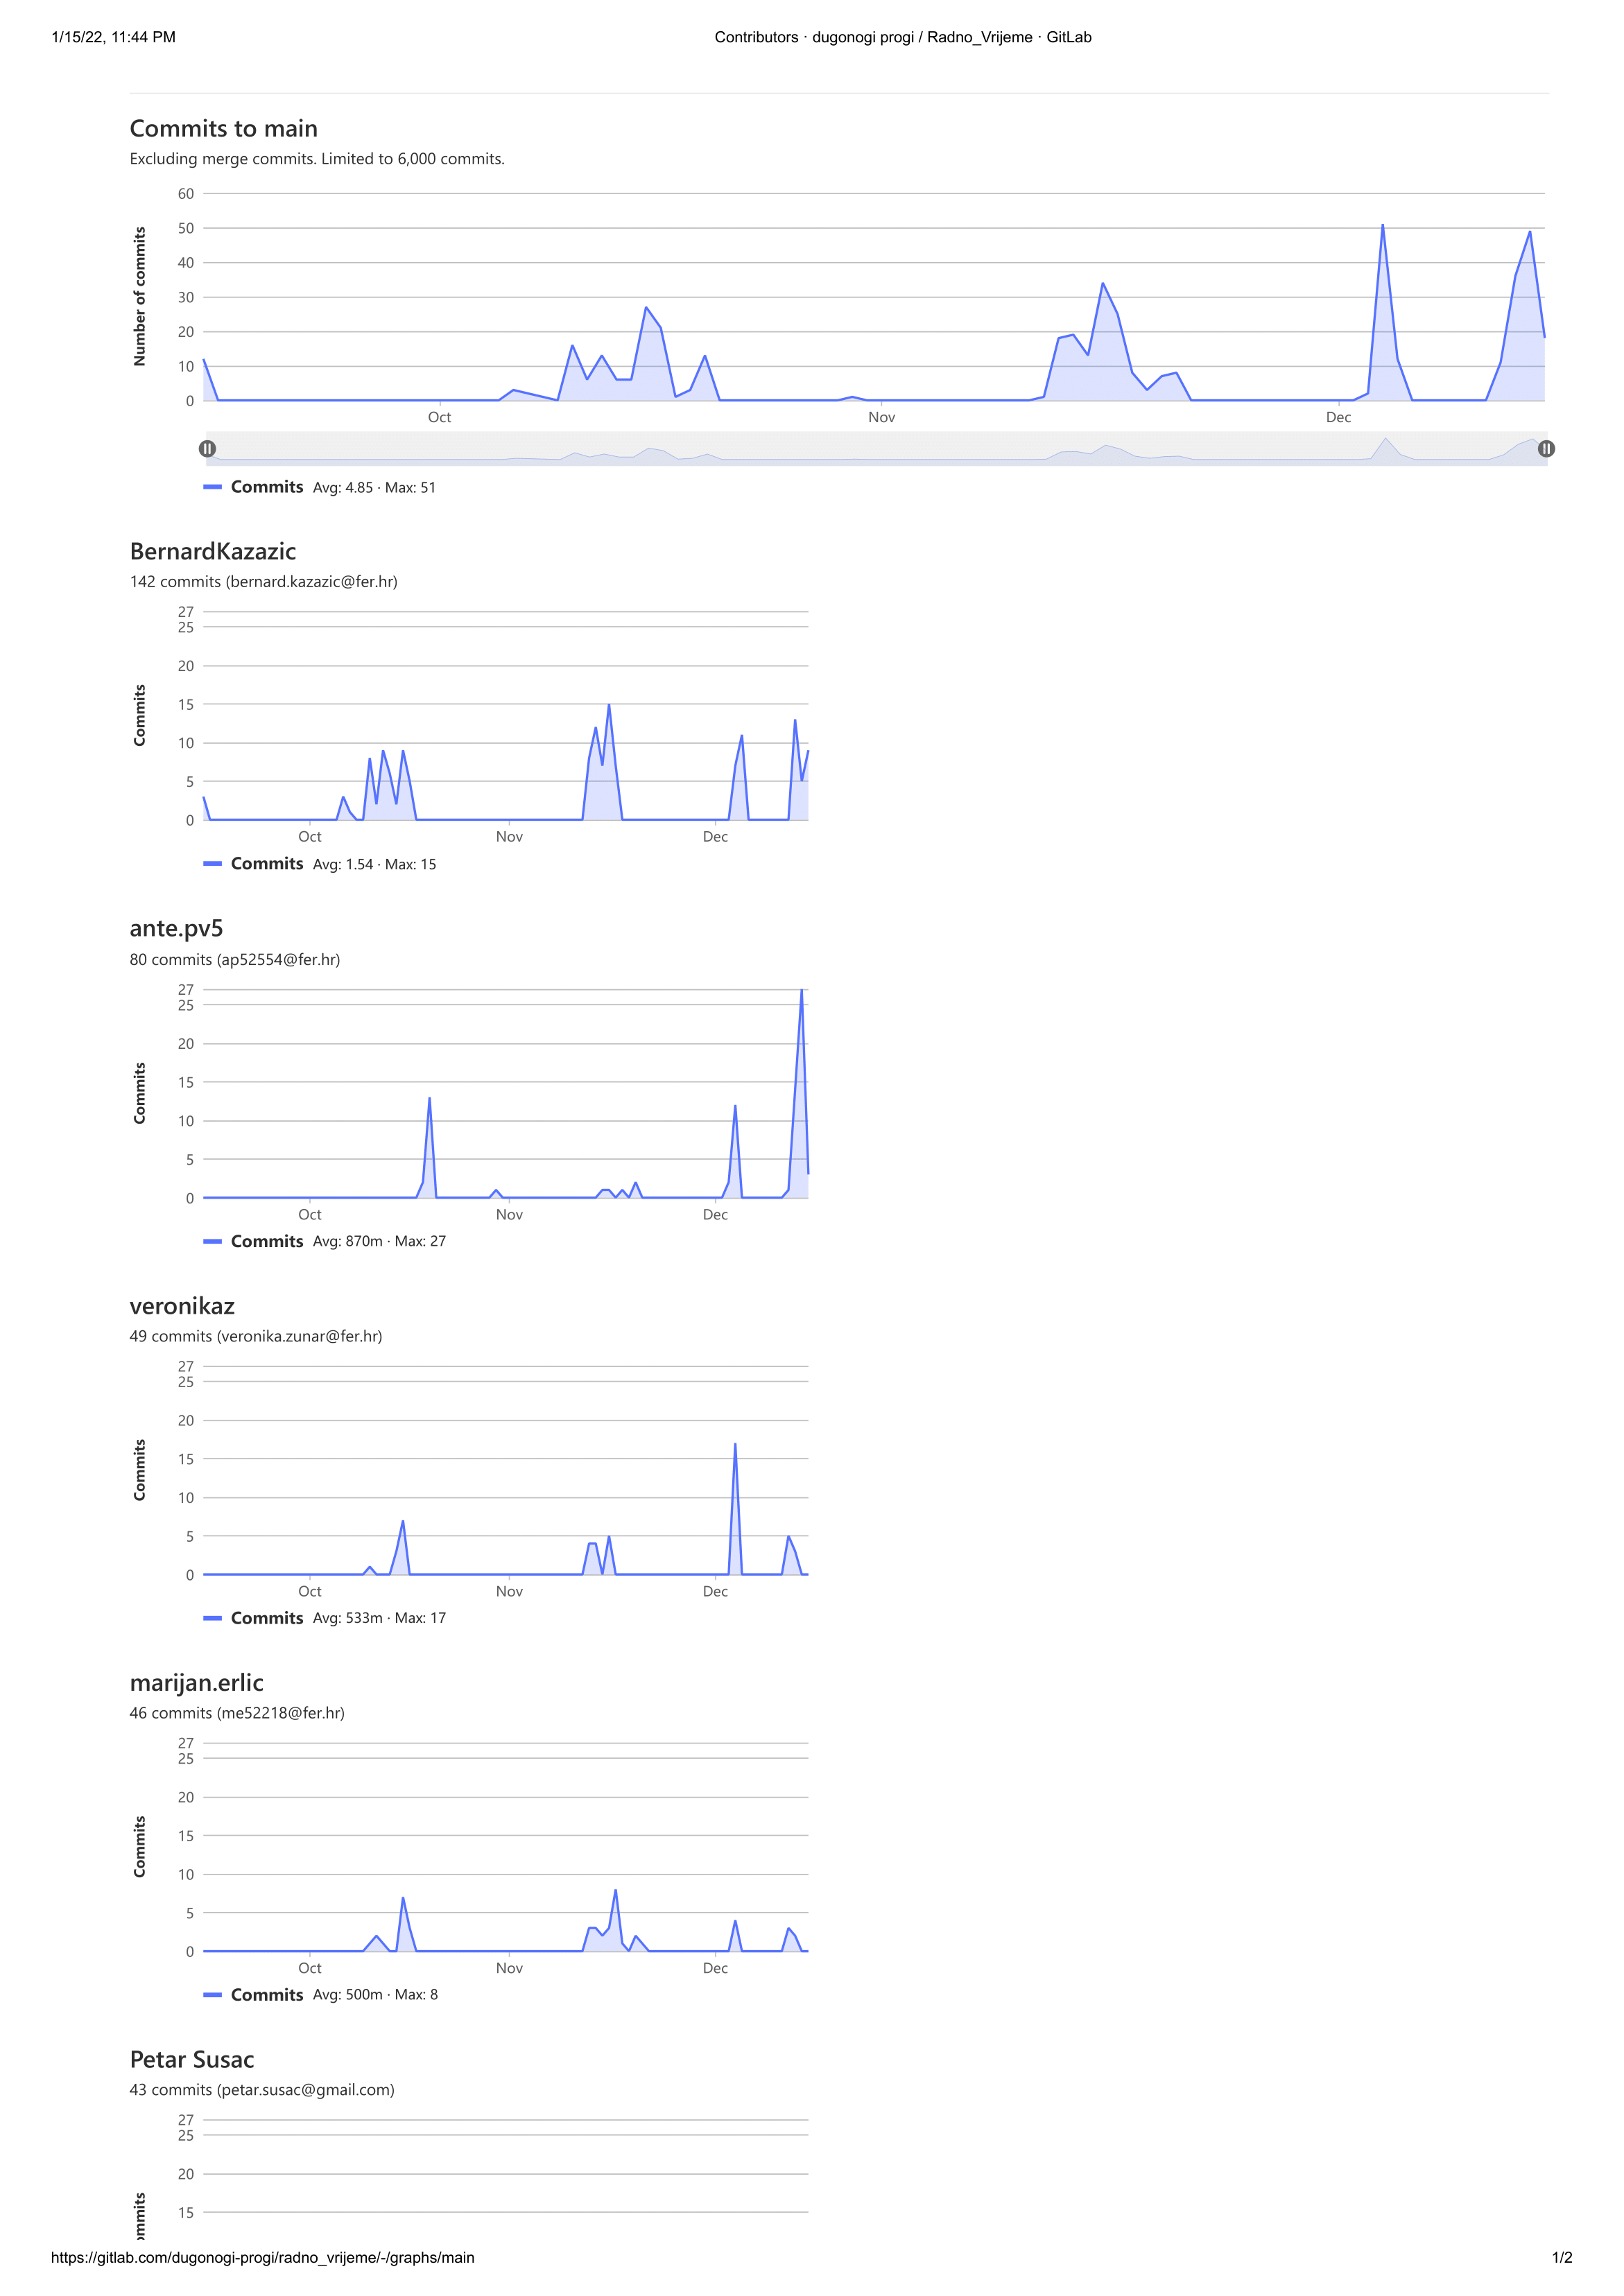
\includegraphics[width=\textwidth]{git1}
					
				\end{figure}
				\begin{figure}[H]
					\centering
					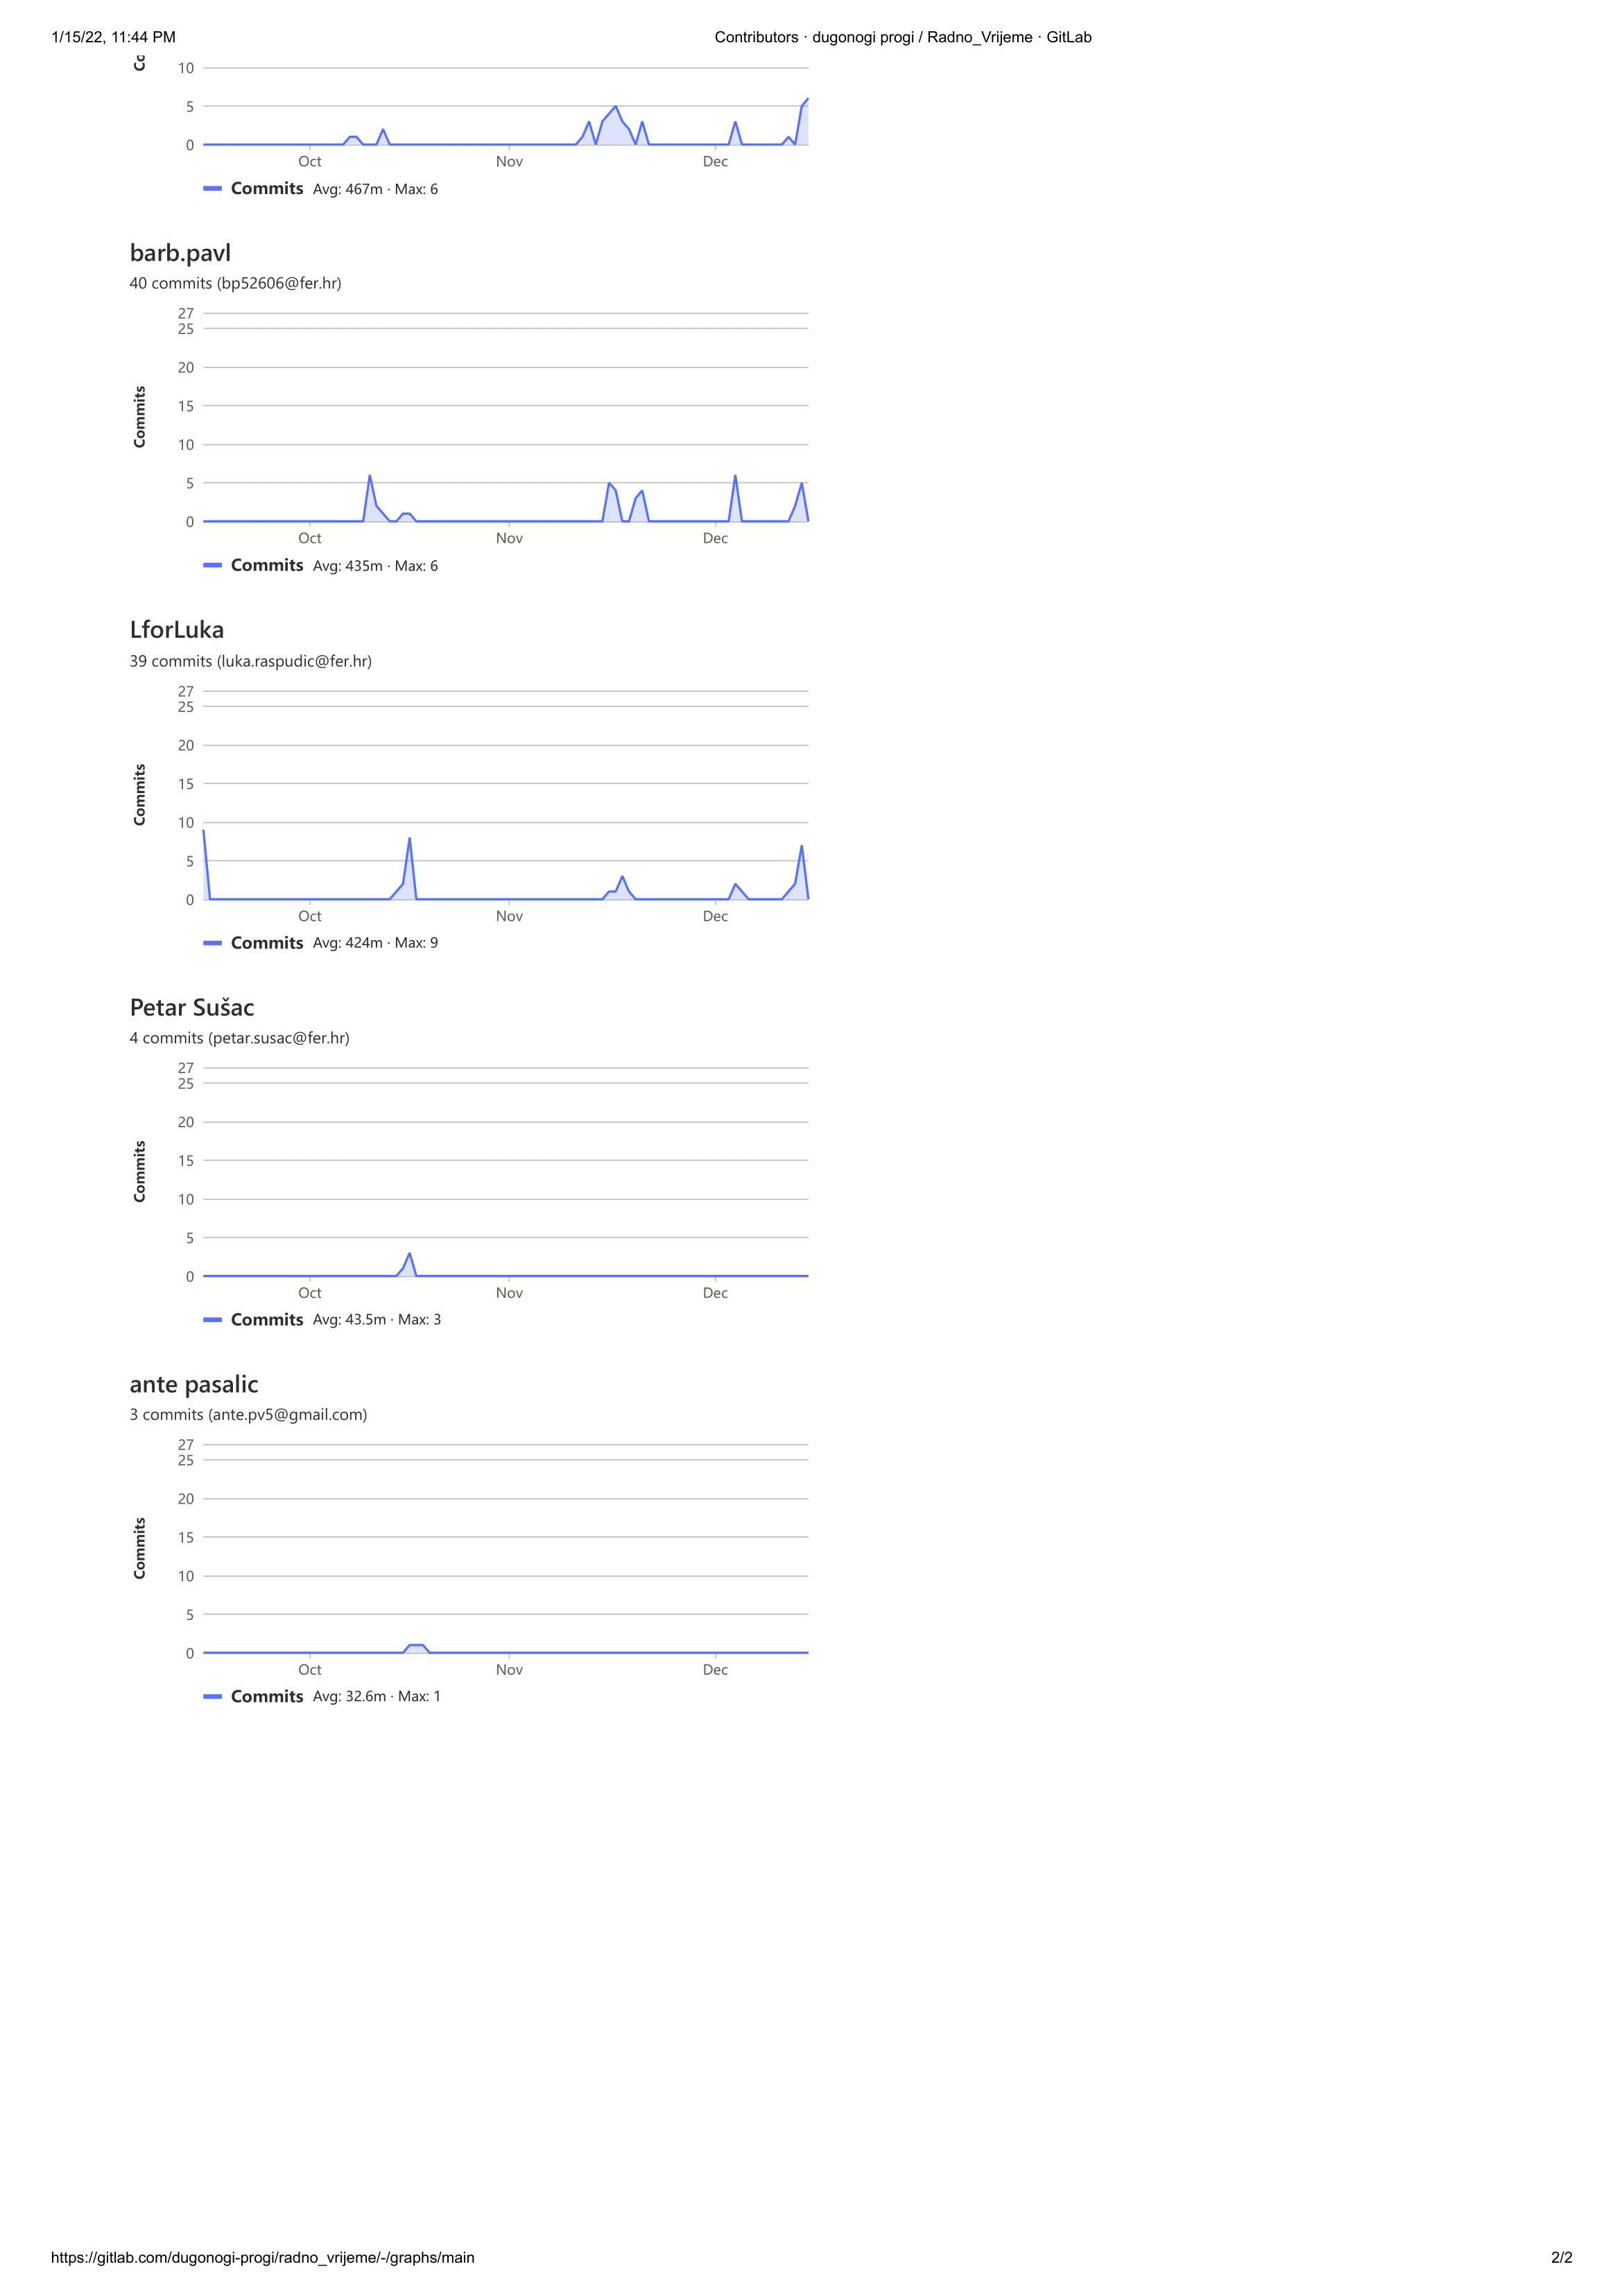
\includegraphics[width=\textwidth]{git2}
					\caption{GitLab dijagram promjena}
				\end{figure}
		
	